Phần cứng bao gồm thiết bị và máy tính điều khiển. Trong đó thiết bị bao gồm 2 khối màn hình và mạch Raspberry Pi 3. Trong mỗi thành phần lại bao gồm các mô đun phần mềm và phần cứng khác nhau (Hình \ref{block-diagram}). Khối máy tính điều khiển của người dùng thực hiện chạy chương trình điều khiển và giao tiếp với mạch Raspberry Pi qua dịch vụ SSH. Tại Raspberry Pi, dịch vụ SSH chạy lệnh tương tác với hệ thống Sysfs của trình điều khiển thiết bị màn hình để điều khiển hoạt động của màn hình. Khối màn hình bao gồm mô đun PCF8574 và màn hình LCD1602 sẽ hoạt động theo sự điều khiển của trình điều khiển trên mạch Raspberry Pi.

\begin{figure}[H]
	\centering
	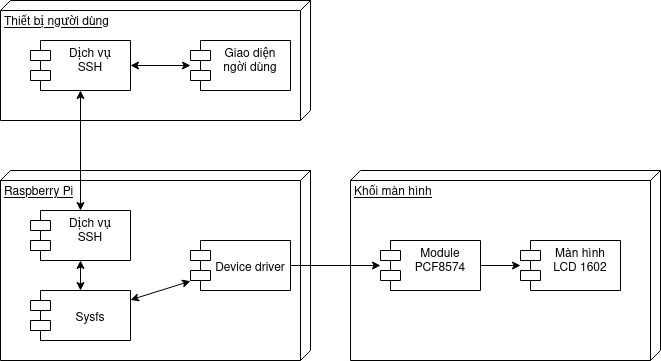
\includegraphics[width=0.8\textwidth]{../images/linux-component.jpg}
	\caption{Sơ đồ khối hệ thống}
	\label{block-diagram}
\end{figure}